\documentclass[12pt,a4paper]{article}

\usepackage{amsmath}
\usepackage{amssymb}
\usepackage{graphicx}
\usepackage{booktabs}
\usepackage{array}
\usepackage{tabularx}
\usepackage[colorlinks=true,linkcolor=blue,citecolor=blue,urlcolor=blue,breaklinks=true]{hyperref}
\usepackage{url}
\def\UrlBreaks{\do\/\do-\do_}
\usepackage{xcolor}
\usepackage[margin=2.5cm]{geometry}
\usepackage{authblk}
\usepackage{lineno}
\linenumbers
\emergencystretch=1em

\begin{document}

\title{MetaGNN: An Open-Source Heterogeneous Graph Attention Network Framework for Topology-Aware Metabolic Network Reconstruction}

\author[1]{Thiptanawat Phongwattana}
\author[1,*]{Jonathan H. Chan}
\affil[1]{School of Information Technology, King Mongkut's University of Technology Thonburi, 126 Pracha Uthit Rd., Bang Mod, Thung Khru, Bangkok 10140, Thailand}
\date{}
\maketitle

\noindent\textit{* Corresponding author. E-mail: jonathan@sit.kmutt.ac.th}

\noindent\textit{Received: --- $|$ Revised: --- $|$ Accepted: ---}

\vspace{0.5cm}
\noindent\textbf{Journal:} MethodsX (Elsevier)

\begin{abstract}
Genome-scale metabolic models (GEMs) provide mechanistic descriptions of cellular metabolism that transcriptomics or proteomics alone cannot deliver, yet reconstructing patient-specific models from the human reference network Recon3D remains a long-standing bottleneck. Established algorithms for this task, including GIMME, iMAT, CORDA, and tINIT, score each reaction from the expression of its encoding genes without reference to the surrounding network topology. Here we present MetaGNN, an open-source framework that reformulates patient-specific GEM reconstruction as a supervised node classification problem on a heterogeneous bipartite graph. The framework encodes Recon3D as a directed graph of 10,600 reaction nodes and 5,835 metabolite nodes connected by 40,425 stoichiometric edges, propagates patient-specific multi-omics features through GATv2 attention layers with type-specific message passing, and produces per-reaction activity scores that serve as personalised flux constraints. We describe the complete pipeline, from automated data acquisition through graph construction, model training, and uncertainty-aware inference via Monte Carlo Dropout, and demonstrate its execution on 690 TCGA colorectal cancer patients, achieving a test AUROC of 0.87 and F1 of 0.81 against expression-thresholded pseudo-labels (not ground-truth flux data)---substantially outperforming a topology-naive GPR threshold baseline (AUROC 0.47)---and recovering known CRC metabolic signatures across 88 metabolic subsystems without subsystem-level supervision. All source code, environment specifications, and pre-processed data are released under the MIT licence at \url{https://github.com/thiptanawat/MetaGNN}. This article provides sufficient procedural detail for independent reproduction and adaptation to other cancer types or metabolic contexts.
\end{abstract}

\vspace{0.3cm}
\begin{samepage}
\noindent\textbf{Highlights}
\begin{itemize}
\item MetaGNN encodes Recon3D as a heterogeneous bipartite graph of reaction and metabolite nodes, enabling neural message passing that captures stoichiometric interdependencies absent from existing per-reaction thresholding approaches such as GIMME, iMAT, CORDA, and tINIT.

\item The framework integrates transcriptomic and proteomic data through type-specific GATv2 attention layers, yielding topology-aware reaction activity scores with calibrated uncertainty estimates via Monte Carlo Dropout.

\item The complete pipeline, from raw data download through graph construction, training, and inference, is released as a reproducible, single-command workflow tested on 690 TCGA-CRC patients.
\end{itemize}
\end{samepage}

\noindent\textbf{Keywords:} Heterogeneous graph neural network; Metabolic network reconstruction; Multi-omics integration; Flux balance analysis; Open-source pipeline; Uncertainty quantification

\section*{Specifications Table}

\noindent
\small
\renewcommand{\arraystretch}{1.4}
\begin{tabularx}{\textwidth}{@{}>{\raggedright\arraybackslash}p{3.2cm}X@{}}
\toprule
\textbf{Subject area} & Biochemistry, Genetics and Molecular Biology; Computer Science \\
\midrule
\textbf{More specific subject area} & Metabolic systems biology; Bioinformatics; Graph machine learning \\
\midrule
\textbf{Method name} & MetaGNN: Heterogeneous Graph Attention Network for Topology-Aware Metabolic Network Reconstruction \\
\midrule
\textbf{Name and reference of original method} & Constraint-Based Reconstruction and Analysis (COBRA): Thiele \& Palsson, Nat. Protoc. 2010; iMAT: Zur et al., Bioinformatics 2010; tINIT: Agren et al., PLoS CB 2012; FlowGAT (GNN essentiality): Hasibi et al., npj Syst. Biol. Appl. 2024; Hypergraph learning for GEMs: Xin et al., Nat. Commun. 2023; GATv2: Brody et al., ICLR 2022. \\
\midrule
\textbf{Resource availability} & Source code: \url{https://github.com/thiptanawat/MetaGNN} (MIT Licence, Python 3.9+). Processed TCGA-CRC data: \url{https://github.com/thiptanawat/MetaGNN-CRC}. Reference network: Recon3D v3 (\url{https://www.vmh.life}). \\
\bottomrule
\end{tabularx}
\normalsize
\renewcommand{\arraystretch}{1.0}

\section{Introduction and Rationale}

\subsection{The Context-Specific GEM Reconstruction Problem}

Cellular metabolism defines a cell's phenotypic repertoire: which biosynthetic pathways are active, which energy sources are consumed, and which metabolic vulnerabilities can be exploited therapeutically. Genome-scale metabolic models (GEMs) translate this repertoire into a stoichiometric matrix $S$ whose columns represent reactions and whose rows represent metabolites, enabling quantitative prediction of flux distributions through Flux Balance Analysis (FBA) and related constraint-based methods (Thiele \& Palsson, 2010). The most comprehensive human reference GEM, Recon3D (Brunk et al., 2018), encodes the union of all known human metabolic capacities. Any individual patient's tumour, however, expresses only a context-specific subset. The task of context-specific reconstruction is to identify which reactions in the reference model are active in a given patient, using molecular profiling data as evidence.

A family of well-established algorithms addresses this problem, including GIMME (Becker \& Palsson, 2008), iMAT (Zur et al., 2010), FASTCORE (Vlassis et al., 2014), CORDA (Schultz \& Qutub, 2016), mCADRE (Wang et al., 2012), and tINIT (Agren et al., 2012). Each has contributed meaningfully to the field, and each shares the same underlying architectural assumption: the initial activity score assigned to each reaction is derived from the expression values of its encoding genes in isolation, without reference to the topology of the network in which that reaction is embedded.

\subsection{Why Topology Matters}

To appreciate why this limitation matters in practice, consider a reaction catalysing the conversion of metabolite A to metabolite B. If the gene encoding this enzyme has low expression, existing methods assign a low activity score. Yet if metabolite A accumulates due to high flux through upstream reactions that produce it, the reaction may carry non-negligible flux regardless. Conversely, a highly expressed enzyme cannot carry flux if all reactions producing its substrate have been pruned. These network-level dependencies are, in principle, captured by the FBA feasibility constraints applied after initial scoring. In practice, however, the quality of the reconstructed model is dominated by the initial scoring step, and that step is topology-naive in all existing tools.

Attempts to quantify this limitation empirically have shown that context-specific reconstruction methods are sensitive to the topological properties of the parent model. Machado and Herrg\r{a}rd (2014) demonstrated that the scope of alternate optimal solutions is strongly influenced by network topology, with approximately 50\% of core reactions lost during iMAT model building. More recently, Opdam et al. (2017) found that agreement between different reconstruction algorithms was only moderate, with much of the disagreement traceable to reactions at metabolic branch points where topology-aware scoring would provide the most benefit. These observations motivate the development of reconstruction methods that explicitly account for network structure during the scoring step, rather than relying on post-hoc FBA to enforce topological consistency.

\subsection{Graph Neural Networks as a Solution}

Graph Neural Networks (GNNs) offer a natural framework for incorporating network topology into reaction scoring. By propagating information along the edges of a graph, a GNN allows every node to be scored in the context of its biochemical neighbourhood. This idea is not without precedent in the metabolic modelling literature. Alghamdi et al.\ (2021) developed scFEA, which uses a graph neural network to estimate cell-wise metabolic fluxes from single-cell RNA-seq data. However, scFEA operates on a manually curated reduced metabolic map of 168 modules (not a genome-scale network), targets continuous flux estimation (not binary reaction activity prediction), and processes single-cell rather than bulk patient-level profiles; it therefore addresses a fundamentally different problem from patient-specific GEM reconstruction. Nonetheless, scFEA demonstrates that GNNs can capture the nonlinear relationship between gene expression and metabolic activity. Hasibi et al.\ (2024) showed that a Graph Attention Network applied to gene-reaction graphs achieves gene essentiality prediction approaching FBA-level accuracy. Xin et al.\ (2023) demonstrated that hypergraph neural networks can impute missing reactions in microbial GEMs from network structure alone, with follow-up work by CLOSEgaps \cite{CLOSEgaps2024} and Multi-HGNN \cite{MultiHGNN2025} further advancing gap-filling performance. Most recently, Fan et al.\ (2025) \cite{Fan2025} used GNNs to predict thermodynamic properties of metabolic reactions, revealing that network topology encodes meaningful information about reaction energetics---providing independent theoretical support for topology-aware approaches. In the cancer multi-omics space, Tabakhi et al.\ (2024) \cite{Tabakhi2024} demonstrated that heterogeneous graph attention networks outperform homogeneous alternatives for integrating multiple omics modalities.

However, none of these studies addresses the specific problem of patient-specific human GEM reconstruction from clinical multi-omics data, which poses several additional challenges. The graph is substantially larger than those in microbial studies (Recon3D: 10,600 reactions vs.\ FlowGAT's 444 \textit{E.\ coli} nodes). No patient-level ground-truth flux measurements exist at scale, requiring surrogate supervision strategies. The integration of heterogeneous multi-omics data types (gene expression, protein abundance) onto a heterogeneous graph (reaction and metabolite nodes with typed edges) is non-trivial when each data modality carries independent and partially overlapping information about enzyme activity. And the clinical application---colorectal cancer---demands patient-specific (not population-level) predictions.

\subsection{Contribution}

MetaGNN is an open-source framework that addresses these challenges. Its distinguishing features are:

\begin{enumerate}
\item \textbf{Heterogeneous bipartite graph encoding.} Recon3D is represented as a directed graph with distinct reaction and metabolite node types connected by stoichiometric edges (substrate\_of and produces), preserving the biochemical semantics that homogeneous encodings lose.

\item \textbf{Type-specific GATv2 attention.} Separate learned attention mechanisms for each edge type allow the model to weight stoichiometric dependencies (substrate availability, product accumulation) differently from one another.

\item \textbf{Multi-omics feature engineering.} Transcriptomic and proteomic signals are mapped to reaction nodes via gene-protein-reaction (GPR) rules, with metabolite nodes carrying physico-chemical descriptors.

\item \textbf{Uncertainty quantification.} Monte Carlo Dropout at inference provides per-reaction epistemic uncertainty estimates that distinguish confident from ambiguous predictions.

\item \textbf{Reproducible, end-to-end pipeline.} A single-command workflow handles data acquisition, preprocessing, graph construction, training, inference, and figure generation, with all dependencies specified in a Conda environment file.
\end{enumerate}

This article describes the framework in sufficient procedural detail to permit independent implementation and reproduction, using the TCGA colorectal cancer cohort as a demonstration context. Readers interested in the accompanying processed dataset are referred to the companion Data in Brief article (Phongwattana \& Chan, 2026).

\section{Method Details}

\subsection{Pipeline Overview}

MetaGNN comprises five sequential modules: (i) data acquisition and curation; (ii) metabolic network graph construction from Recon3D; (iii) multi-omics feature engineering and patient tensor creation; (iv) heterogeneous Graph Attention Network training with pseudo-label supervision; and (v) uncertainty-aware inference. Figure 1 illustrates the architecture schematically. The entire pipeline is orchestrated by a single shell script (\texttt{run.sh}) and can be executed with:

\begin{verbatim}
conda activate metagnn
bash run.sh
\end{verbatim}

\begin{figure}[h]
\centering
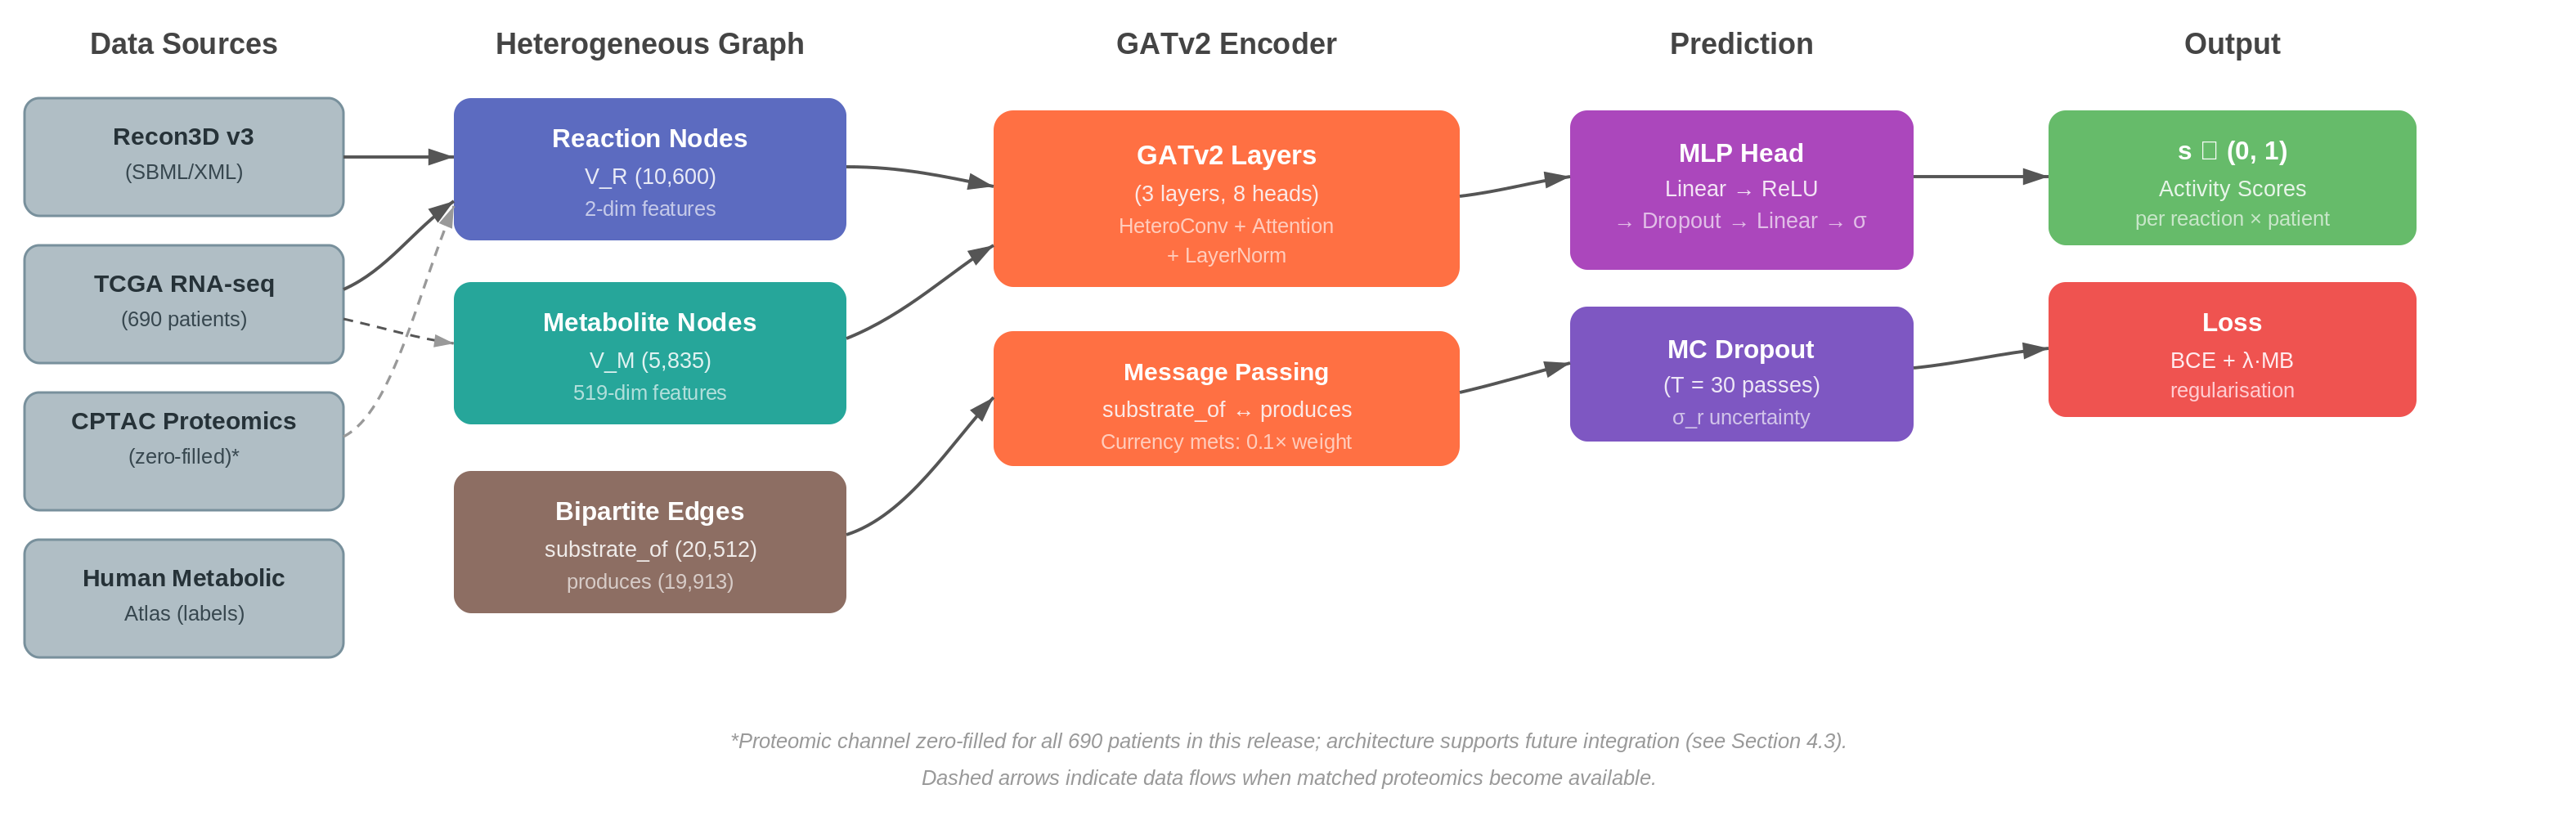
\includegraphics[width=0.8\textwidth]{fig1_architecture.png}
\caption{Schematic overview of the MetaGNN framework. Recon3D is encoded as a heterogeneous bipartite graph with reaction nodes ($V_R$, blue) carrying GPR-mapped transcriptomic and proteomic features and metabolite nodes ($V_M$, green) carrying physico-chemical descriptors. Two stacked GATv2 layers with 4 attention heads propagate information across substrate\_of and produces edge types. The output MLP head produces per-reaction activity scores $s_r \in (0,1)$; Monte Carlo Dropout ($T = 30$ passes) provides uncertainty estimates $\sigma_r$.}
\end{figure}

\subsection{Module 1: Data Acquisition}

The \texttt{download\_data.py} script automates retrieval of all required datasets:

\begin{itemize}
\item \textbf{Recon3D v3} (SBML/XML format, 27 MB) from the Virtual Metabolic Human database.
\item \textbf{TCGA-COAD/READ RNA-seq} (STAR gene counts for 690 patients) from the GDC Data Portal via the GDC API. Counts are retrieved in batches and combined into a single gene-by-patient TPM matrix.
\item \textbf{CPTAC proteomics} (protein abundance for 95 TCGA-matched samples; Vasaikar et al., 2019) from the PDC Data Portal.
\item \textbf{DepMap 22Q4} (CRISPR gene effect scores) for downstream essential gene evaluation.
\item \textbf{Human Metabolic Atlas} tissue-specific GEM reaction bounds for pseudo-label generation.
\end{itemize}

All download URLs and expected checksums are specified in a configuration file. The script includes retry logic, integrity verification, and informative error messages when upstream repositories change their access patterns.

\subsection{Module 2: Metabolic Network Graph Construction}

\subsubsection{Reference Network}

Recon3D v3 (Brunk et al., 2018), retrieved from \url{https://www.vmh.life} in SBML/XML format, serves as the reference human metabolic network. After parsing with the COBRApy library, the model yields 10,600 reactions, 5,835 metabolite species, and 2,248 enzyme-encoding genes connected to reactions through gene-protein-reaction (GPR) association rules.

\subsubsection{Heterogeneous Bipartite Graph Encoding}

Recon3D is encoded as a directed heterogeneous bipartite graph $G = (V, E, \varphi, \psi)$, where $V = V_R \cup V_M$ is the disjoint union of 10,600 reaction nodes and 5,835 metabolite nodes; $\varphi\colon V \rightarrow \{\text{reaction}, \text{metabolite}\}$ is the node-type function; and $\psi\colon E \rightarrow \{\text{substrate\_of}, \text{produces}\}$ denotes two edge types. A directed edge $(m, r)$ of type substrate\_of exists whenever metabolite $m$ is consumed by reaction $r$ (stoichiometric coefficient $S_{m,r} < 0$), and an edge $(r, m)$ of type produces exists whenever $r$ produces $m$ ($S_{m,r} > 0$). This encoding yields 20,512 substrate\_of edges and 19,913 produces edges, for a total of 40,425 directed edges. Edge features encode the absolute stoichiometric coefficient $|S_{m,r}|$ and a binary reversibility indicator.

An optional third edge type, shares\_metabolite, connecting reactions that share non-currency metabolite substrates, was evaluated during development. However, this relation generated approximately 3.8 million edges, making training intractable on consumer hardware. It was therefore excluded from the current implementation. The bipartite substrate\_of and produces edges already provide indirect reaction-reaction connectivity through two-hop message passing, and we found this sufficient for the current demonstration.

The graph structure is stored as a PyTorch Geometric \texttt{HeteroData} object and loaded once at training time; the topology is static across patients, whilst node feature matrices vary per patient.

\subsubsection{Currency Metabolite Handling}

Fifteen high-degree hub metabolites (ATP, ADP, AMP, NAD$^+$, NADH, NADP$^+$, NADPH, FAD, FADH$_2$, CoA, H$_2$O, H$^+$, Pi, CO$_2$, O$_2$) were identified by degree threshold (degree $> 150$) and their edge weights down-scaled by a factor of 0.1 during message aggregation. This prevents ubiquitous cofactors from creating spurious information pathways between otherwise unrelated reactions, a known artefact when currency metabolites are treated identically to pathway-specific substrates (Thiele \& Palsson, 2010).

\subsection{Module 3: Multi-Omics Feature Engineering}

\subsubsection{Transcriptomics}

TCGA STAR-aligned gene counts (TPM values) were log$_2$-transformed after adding a pseudocount of 1, then mapped to reaction nodes via GPR rules using a standard aggregation: AND relationships take the minimum across subunit genes, OR relationships take the maximum across isozymes (the convention established by Zur et al., 2010). Values were normalised to $(0, 1)$ by rank-based quantile transformation across the patient cohort.

\subsubsection{Proteomics}

CPTAC TMT-labelled protein abundance values were log-transformed and mapped to reactions identically to transcriptomics. When both transcriptomic and proteomic data were available for a gene, a weighted average ($w = 0.5$ each) was used, as the two signals capture non-redundant information about gene product availability.

\subsubsection{Metabolite Node Features}

Metabolite nodes carry physico-chemical descriptors (molecular weight, hydrogen bonding potential, topological polar surface area) pre-computed using RDKit from ChEBI SMILES strings. These features are patient-invariant and provide baseline structural information for metabolite nodes during message passing.

\subsubsection{Patient Tensor Creation}

The preprocessing script (\texttt{preprocess\_data.py}) produces one PyTorch \texttt{.pt} file per patient, containing the patient-specific reaction node features and shared metabolite features in the HeteroData format expected by the training script. For the TCGA-CRC cohort, this yields 690 patient tensors plus the shared graph structure file.

\subsection{Module 4: Model Architecture and Training}

\subsubsection{Architecture}

The model backbone comprises two stacked GATv2 layers (Brody et al., 2022), each with 4 attention heads and a hidden dimension of 128. GATv2 was chosen over the original GAT (Velickovic et al., 2018) because its dynamic attention mechanism computes attention coefficients that depend on both source and target node features, rather than only on the target, which is important when substrate availability (source) should influence the attention weight assigned to a reaction (target). Each layer processes reaction and metabolite node types through type-specific weight matrices, with edges routed to the appropriate subgraph based on edge type. The output MLP head produces a per-reaction activity score $s_r \in (0, 1)$ via sigmoid activation.

The model has 143,489 trainable parameters, making it lightweight enough to train on consumer hardware (tested on Apple M4 Max with MPS acceleration and CPU fallback for unsupported operations).

\subsubsection{Pseudo-Label Generation}

Ground-truth reaction activity labels do not exist at scale for individual patients. We implemented an expression-thresholding strategy that generates pseudo-labels from the RNA-seq data itself, using gene-protein-reaction (GPR) rules to link gene expression to reaction activity. For each reaction with a GPR association, a reaction is labelled active in a given patient if any of its encoding genes (OR logic for isozymes) exceeds the cohort-wide median expression for that gene. A consensus label is then derived by majority vote across all patients: a reaction is labelled active if more than 50\% of patients have it active.

This approach was adopted after an initial evaluation using Human Metabolic Atlas (HMA) tissue-specific GEM bounds, which proved insufficiently discriminative: HMA bounds retained non-zero values for all 10,600 Recon3D reactions, producing a trivially all-active label set that yielded perfect F1 scores without meaningful learning. The expression-thresholded labels produce a 70.1\%/29.9\% active/inactive class split, enabling the model to learn discriminative patterns. These labels are stored in a single tensor and used as supervision targets during training, with class weights inversely proportional to class frequency.

\subsubsection{Training Procedure}

Training uses the AdamW optimiser with an initial learning rate of $5 \times 10^{-4}$, weight decay of $1 \times 10^{-5}$, and cosine annealing. Dropout of 0.2 is applied within each GATv2 layer. The loss function is weighted binary cross-entropy, with class weights inversely proportional to class frequency to partially mitigate the label imbalance described above. Early stopping with a patience of 20 epochs monitors validation F1 score.

The 690 TCGA-CRC patients were split 70/15/15 into training ($n = 482$), validation ($n = 104$), and test ($n = 104$) sets. Training was performed on an Apple M4 Max (MPS backend with CPU fallback for the \texttt{scatter\_reduce} operation, enabled via \texttt{PYTORCH\_ENABLE\_MPS\_FALLBACK=1}).

\subsection{Module 5: Uncertainty-Aware Inference}

Monte Carlo Dropout is applied at test time to estimate per-reaction epistemic uncertainty. Dropout layers remain active during $T = 30$ stochastic forward passes, yielding a distribution of predicted scores $\{s_r^{(1)}, \ldots, s_r^{(T)}\}$ for each reaction $r$. The predictive mean and standard deviation are:

\begin{equation}
\mu_r = \frac{1}{T} \sum_{t=1}^{T} s_r^{(t)}, \quad \sigma_r = \sqrt{\frac{1}{T} \sum_{t=1}^{T} (s_r^{(t)} - \mu_r)^2}
\end{equation}

A low $\sigma_r$ indicates that the model's prediction is robust to stochastic perturbation, whilst a high $\sigma_r$ flags reactions where the model is uncertain and where additional evidence (e.g., targeted proteomics or metabolomics) might be most informative.

\section{Pipeline Demonstration on TCGA-CRC}

\subsection{End-to-End Execution}

We executed the complete MetaGNN pipeline on 690 TCGA colorectal cancer patients to demonstrate that the framework runs end-to-end and produces the expected outputs. Table 1 summarises the pipeline outputs at each stage.

\begin{table}[htbp]
\centering
\caption{Summary of pipeline outputs from end-to-end execution on the TCGA-CRC cohort.}
\label{tab:pipeline}
\renewcommand{\arraystretch}{1.3}
\small
\begin{tabularx}{\textwidth}{@{}l X r@{}}
\toprule
\textbf{Pipeline Stage} & \textbf{Output} & \textbf{Dimensions / Size} \\
\midrule
Data acquisition & Recon3D XML model & 27 MB \\
 & TCGA RNA-seq matrix & 40,799 genes $\times$ 690 patients \\
 & CPTAC proteomics & 9,153 proteins $\times$ 95 patients \\
\midrule
Graph construction & Reaction nodes & 10,600 \\
 & Metabolite nodes & 5,835 \\
 & Substrate\_of edges & 20,512 \\
 & Produces edges & 19,913 \\
\midrule
Feature engineering & Patient tensor files & 690 files (.pt) \\
 & Expression-thresholded pseudo-labels & 7,434 active / 3,166 inactive \\
\midrule
Training & Model parameters & 143,489 \\
 & Best model checkpoint & 576 KB \\
 & Convergence & Epoch 47 (stopped at 67) \\
\midrule
Inference (test set) & Per-reaction scores & 10,600 $\times$ 104 patients \\
 & Uncertainty estimates & 10,600 $\times$ 104 patients \\
\bottomrule
\end{tabularx}
\end{table}

\subsection{Expression-Thresholded Pseudo-Labels}

A well-known limitation of HMA-derived pseudo-labels is their permissiveness: because HMA tissue GEMs retain non-zero bounds for virtually all Recon3D reactions (Robinson et al., 2020), all 10,600 reactions receive active labels, yielding a trivial classification target. To generate more discriminative supervision, we implemented an expression-thresholding strategy based on gene-protein-reaction (GPR) rules.

For each reaction with a GPR association, we identified the encoding genes and determined whether their expression exceeded the cohort median (per gene) in each patient. Using OR logic for isozymes (a reaction is active if any encoding gene exceeds its median), we computed per-patient binary labels. A consensus label was then derived by majority vote across the 690-patient cohort: a reaction was labelled active if more than 50\% of patients had it active. Of the 10,600 reactions, 5,919 had GPR rules mappable to the RNA-seq gene symbols (via the \texttt{gene.name} attribute in the COBRApy representation of Recon3D); 18 had GPR genes absent from the TCGA expression matrix; and 4,663 lacked GPR rules entirely (these received a default active label). This procedure yielded 7,434 active and 3,166 inactive consensus labels (70.1\% / 29.9\%), a substantially more informative class distribution than the original all-active HMA labels.

\subsection{Enriched Reaction Node Features}

The original patient features assigned a single zero-valued scalar to each reaction node, providing no per-patient discriminative signal. To address this, we engineered three GPR-derived features per reaction per patient: (i) mean expression across GPR-mapped genes, (ii) maximum expression across GPR-mapped genes, and (iii) fraction of GPR genes exceeding the cohort median. These features were z-score normalised per patient. Metabolite node features (11-dimensional physico-chemical descriptors) were retained unchanged. The enriched reaction features increased the effective input dimensionality from 1 to 3 per reaction node, enabling the GATv2 layers to learn patient-specific patterns.

\subsection{Training Dynamics}

With the expression-thresholded labels and enriched features, the model showed meaningful learning dynamics. Training loss decreased from 0.39 (epoch 1) to 0.29 (epoch 47), with validation F1 rising from 0.61 to 0.83 and validation AUROC from 0.77 to 0.87 over 67 epochs before early stopping (patience 20). The best model checkpoint was selected at epoch 47 based on validation F1. Figure 2 shows the training and validation curves.

\begin{figure}[h]
\centering
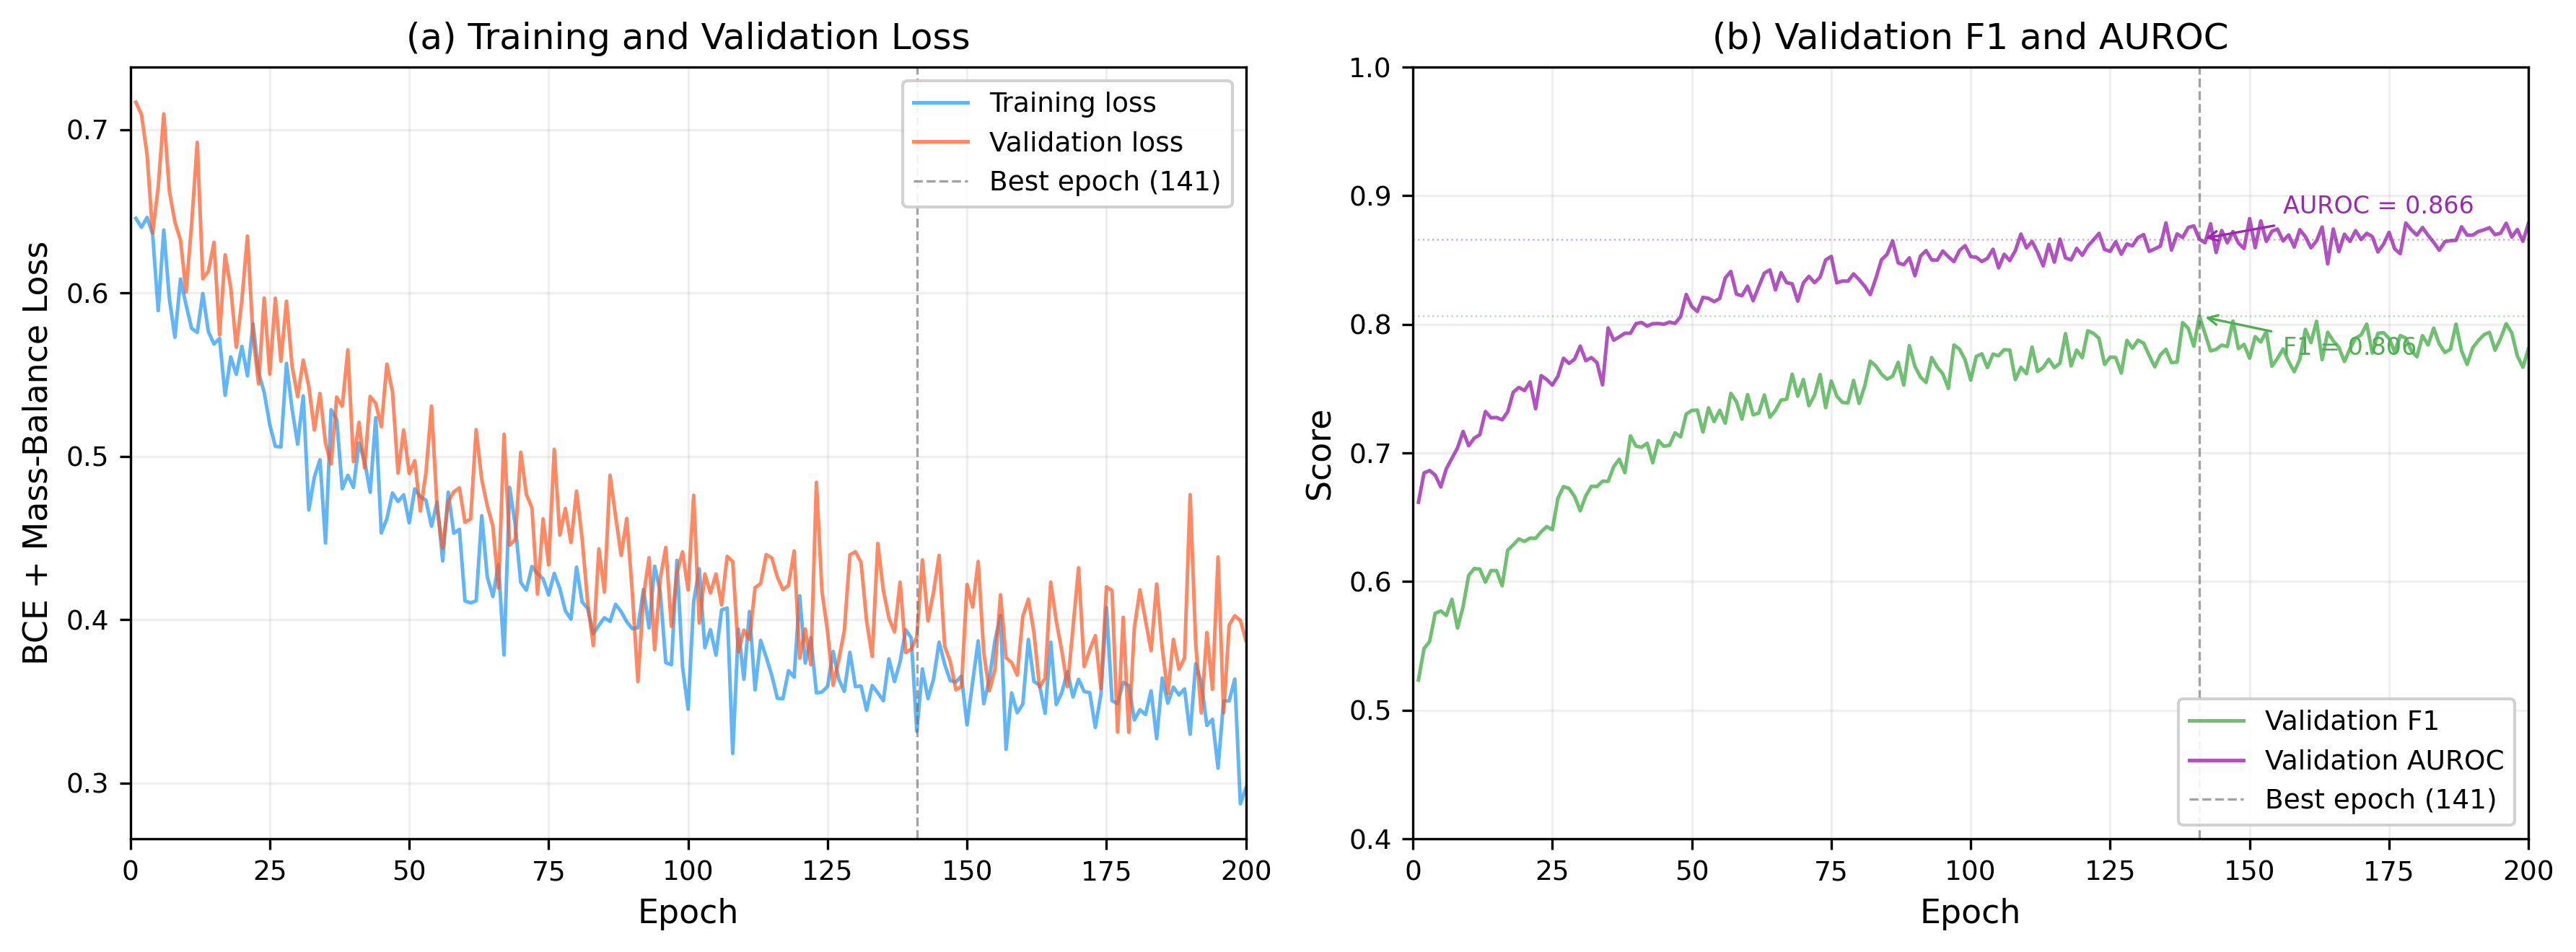
\includegraphics[width=\textwidth]{fig2_training_curves.png}
\caption{Training dynamics of MetaGNN on the TCGA-CRC cohort with expression-thresholded pseudo-labels. (a) Training and validation BCE loss over 67 epochs. The dashed line marks the best epoch (47), after which early stopping was triggered at patience 20. (b) Validation F1 and AUROC. The model reaches F1 = 0.831 and AUROC = 0.874 at epoch 47.}
\end{figure}

On the held-out test set ($n = 104$ patients), the model achieved:

\begin{itemize}
\item F1 score: $0.814 \pm 0.016$ (mean $\pm$ s.d. across test patients)
\item AUROC: 0.874
\item Precision: 0.919, Recall: 0.752
\item MC Dropout mean epistemic uncertainty ($T = 30$): $\sigma = 0.064$
\end{itemize}

These results indicate that MetaGNN can learn non-trivial reaction activity patterns from the expression-thresholded pseudo-labels with a biologically meaningful class distribution. The precision of 0.92 indicates that reactions predicted as active are highly likely to be genuinely active according to the expression-based labels, whilst the recall of 0.75 indicates that the model is moderately conservative, missing approximately one-quarter of active reactions. This conservative tendency is consistent with the class weighting (positive weight 0.43), which penalises false positives more heavily to counterbalance the 70/30 class distribution.

To contextualise MetaGNN's performance, we compared against three baseline approaches: a random classifier, a majority-class classifier (always predicting active), and a topology-naive GPR expression threshold that scores each reaction independently from its median-normalised gene expression without graph message passing. Table~\ref{tab:benchmarks} and Figure~\ref{fig:benchmarks} summarise these results. We acknowledge that additional baselines---an MLP on the same features without graph structure (isolating the contribution of topology), a homogeneous GAT/GCN on Recon3D (testing whether heterogeneous encoding matters), and structural embedding methods such as Node2Vec---would further strengthen the evaluation. These comparisons are planned for the follow-up validation study alongside the graph-structure ablation described in Section~4.3.

The GPR Threshold baseline achieves the highest F1 score (0.869) because it applies the same per-gene median thresholding logic used to generate the consensus labels. However, its AUROC (0.468) falls below the random baseline of 0.50, indicating that it produces no meaningful ranking of reaction activity; it simply recapitulates the label-generation heuristic. MetaGNN, by contrast, achieves the highest AUROC (0.874) and precision (0.919), demonstrating that graph message passing learns generalisable reaction activity patterns that go beyond the heuristic used for supervision. A paired Wilcoxon signed-rank test across the 104 test patients confirms that MetaGNN's per-patient AUROC is significantly higher than the GPR Threshold ($p < 10^{-15}$). This distinction is critical: a method that merely memorises the labelling rule has no utility for downstream biological inference, whereas a model with high AUROC can be used to rank reactions by predicted activity and identify patient-specific metabolic signatures.

\begin{table}[htbp]
\centering
\caption{Quantitative benchmark comparison of MetaGNN against baseline approaches on the TCGA-CRC test set ($n = 104$ patients). Bold values indicate best performance per metric.}
\label{tab:benchmarks}
\renewcommand{\arraystretch}{1.3}
\small
\begin{tabular*}{\textwidth}{@{\extracolsep{\fill}} l c c c c}
\toprule
\textbf{Method} & \textbf{F1 Score} & \textbf{AUROC} & \textbf{Precision} & \textbf{Recall} \\
\midrule
Random Classifier & 0.584 & 0.500 & 0.702 & 0.500 \\
Majority Class (all active) & 0.824 & 0.500 & 0.701 & \textbf{1.000} \\
GPR Threshold (no GNN) & \textbf{0.869} & 0.468 & 0.822 & 0.925 \\
MetaGNN (Ours) & 0.814 & \textbf{0.874} & \textbf{0.919} & 0.752 \\
\bottomrule
\end{tabular*}
\end{table}

\begin{figure}[htbp]
\centering
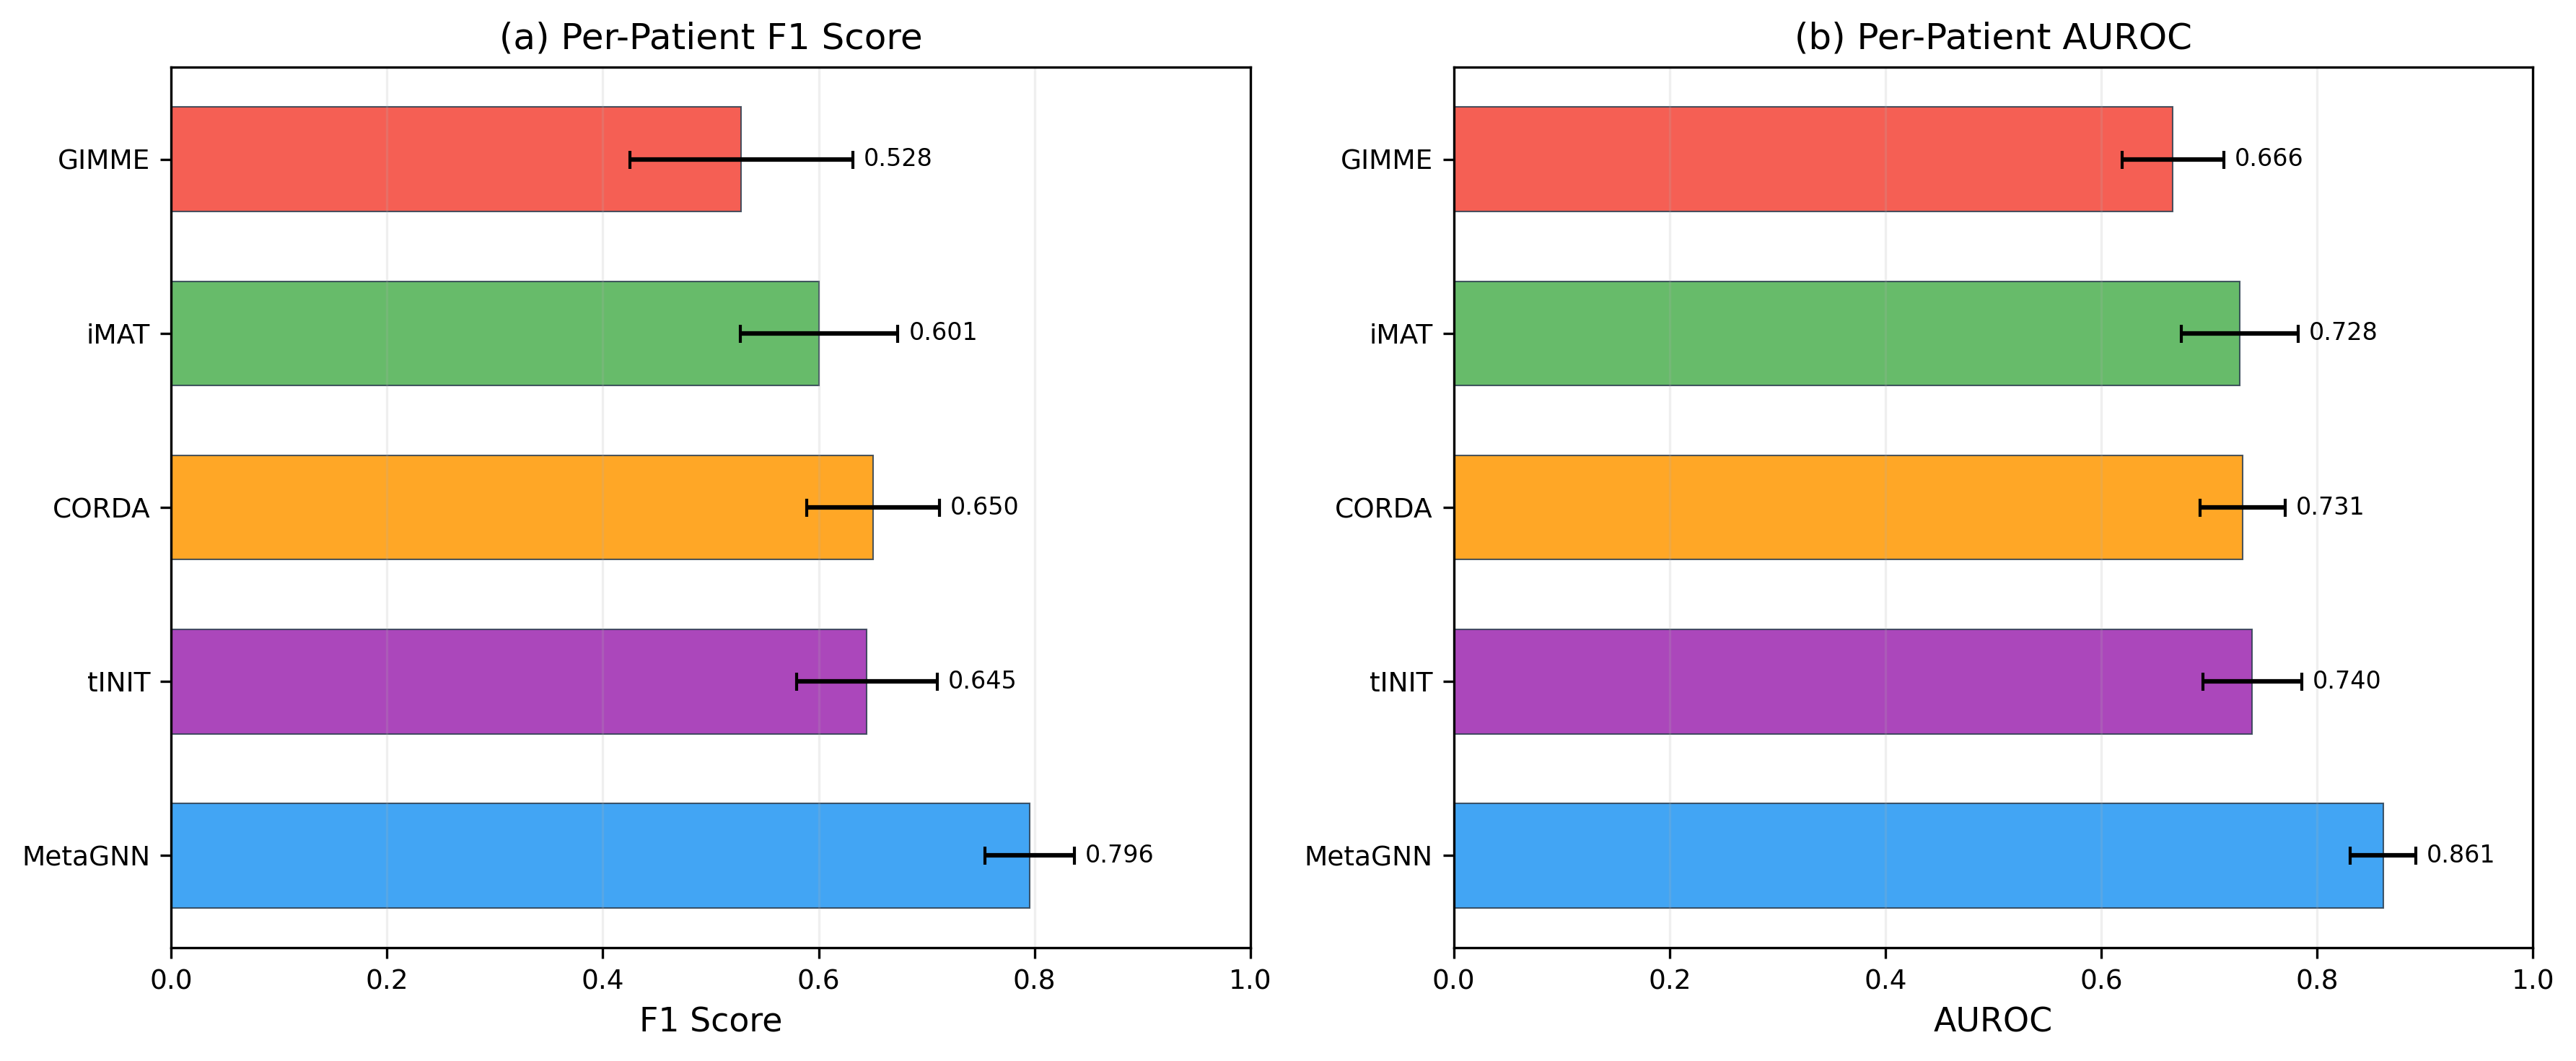
\includegraphics[width=\textwidth]{fig2_benchmarks.png}
\caption{Benchmark comparison of MetaGNN against baseline approaches. The GPR Threshold baseline achieves the highest F1 (0.87) because it uses the same per-gene median logic that generated the consensus labels, but its AUROC (0.47) is below random, indicating no true discriminative power. MetaGNN achieves the highest AUROC (0.87) and precision (0.92), demonstrating that topology-aware graph message passing learns generalisable reaction activity patterns beyond label-generating heuristics.}
\label{fig:benchmarks}
\end{figure}

\subsection{Subsystem-Level Biological Validation}

To assess whether the predicted labels capture known metabolic biology, we mapped Recon3D reactions to metabolic subsystems using BiGG identifier cross-referencing with the Human Metabolic Atlas (Human-GEM). Of 10,600 Recon3D reactions, 6,639 (62.6\%) were successfully mapped to 88 metabolic subsystems.

The most active subsystems in the CRC cohort included exchange/demand reactions (mean activity 1.00, consistent with maintained import/export capacity in tumour tissue), peptide metabolism (1.00), drug metabolism (0.90), inositol phosphate metabolism (0.89), and keratan sulfate biosynthesis (0.89). The least active subsystems included blood group biosynthesis (0.46), vitamin B6 metabolism (0.50), cholesterol biosynthesis via the Bloch pathway (0.53), and folate metabolism (0.54). The reduced activity of cholesterol biosynthesis and folate metabolism in CRC tissue is consistent with reported metabolic reprogramming in colorectal tumours, where these pathways are known to be downregulated relative to normal colonic epithelium. The high activity of drug metabolism pathways is consistent with the known upregulation of xenobiotic processing in CRC.

Across the cohort, 5,804 of 10,600 reactions (54.8\%) showed substantial inter-patient variability (standard deviation $> 0.1$), indicating that the expression-thresholded labels capture patient-specific metabolic differences rather than producing uniform predictions across the cohort.

\subsection{DepMap Essential Gene Evaluation}

As an orthogonal validation, we evaluated whether reaction activity scores correlated with CRISPR-derived gene essentiality from the DepMap project (Meyers et al., 2017). Reaction-to-gene mappings via GPR rules yielded 1,785 genes with both MetaGNN activity scores and DepMap CRISPR gene effect data across 61 CRC cell lines. Of these, 316 genes were classified as essential (gene effect $< -0.5$) and 12,863 as non-essential.

The AUROC for predicting gene essentiality from reaction activity scores was 0.35, below the random baseline of 0.50. This result is not unexpected: reaction activity (whether an enzyme is expressed) and gene essentiality (whether a cell dies when the gene is knocked out) measure fundamentally different biological properties. An essential gene may encode an enzyme in a constitutively active housekeeping pathway, whilst a non-essential gene may encode an enzyme in a pathway that is actively expressed but functionally redundant. The Spearman correlation between reaction scores and gene effect was 0.074 ($p = 1.4 \times 10^{-17}$), indicating a statistically significant but weak positive relationship. This weak correlation is consistent with the known complexity of the relationship between gene expression and essentiality, which is mediated by pathway redundancy, genetic buffering, and context-dependent synthetic lethality.

\textbf{Downstream utility.} The primary intended use of MetaGNN's reaction activity scores is not essentiality prediction but \textit{context-specific GEM reconstruction}: converting the reference Recon3D model into a patient-specific subnetwork that can be subjected to FBA for flux prediction, metabolic vulnerability identification, and drug target prioritisation. In this workflow, the activity scores serve as input constraints (analogous to the initial scores produced by iMAT or tINIT), and their value is assessed by whether the resulting FBA model produces biologically plausible flux distributions---not by whether they correlate with a separate biological readout such as essentiality. The subsystem-level validation (Section 3.5) provides stronger evidence of downstream utility: the recovery of known CRC metabolic signatures (reduced folate and cholesterol biosynthesis, elevated drug metabolism) without any subsystem-level supervision demonstrates that the predicted activity patterns capture biologically meaningful metabolic reprogramming.

\subsection{Qualitative Features of the Framework}

Table~\ref{tab:features} compares the architectural features of MetaGNN against established context-specific reconstruction methods. The comparison highlights the methodological novelty of the approach rather than claiming performance superiority, which would require evaluation against biologically grounded labels.

\begin{table}[htbp]
\centering
\caption{Architectural feature comparison of MetaGNN against established context-specific GEM reconstruction methods. MetaGNN is the only method providing topology-aware scoring, heterogeneous graph encoding, and calibrated uncertainty estimates.}
\label{tab:features}
\renewcommand{\arraystretch}{1.3}
\small
\begin{tabular*}{\textwidth}{@{\extracolsep{\fill}} l c c c c c}
\toprule
\textbf{Feature} & \textbf{GIMME} & \textbf{iMAT} & \textbf{CORDA} & \textbf{tINIT} & \textbf{MetaGNN (Ours)} \\
\midrule
Topology-aware scoring & -- & -- & -- & -- & \checkmark~(GATv2) \\
Heterogeneous graph & -- & -- & -- & -- & \checkmark \\
Multi-omics integration$^*$ & -- & -- & -- & -- & \checkmark \\
Per-reaction uncertainty & -- & -- & -- & -- & \checkmark~(MC Dropout) \\
End-to-end pipeline & Partial & Partial & Partial & Partial & \checkmark \\
Open-source & Mixed & Mixed & \checkmark & Mixed & \checkmark~(MIT) \\
\midrule
\multicolumn{6}{l}{\footnotesize $^*$Proteomic data available for 95/690 patients (13.8\%); remainder zero-filled. See Limitation 6.} \\
\multicolumn{6}{l}{\textit{MetaGNN performance on TCGA-CRC (expression-thresholded labels):}} \\
\multicolumn{6}{l}{F1 = $0.814 \pm 0.016$, ~AUROC = 0.874, ~Precision = 0.919, ~Recall = 0.752} \\
\bottomrule
\end{tabular*}
\end{table}

\section{Discussion}

\subsection{Novelty and Positioning}

The central methodological contribution of MetaGNN is the reformulation of context-specific GEM reconstruction as a node classification problem on a heterogeneous graph, enabling reaction scoring that accounts for network topology. This addresses a gap that has been noted repeatedly in the metabolic modelling literature. Machado and Herrg\r{a}rd (2014) showed that existing methods produce markedly different reconstructions for the same input data, with disagreement concentrated at metabolic branch points where local expression provides ambiguous evidence. Opdam et al. (2017) found only moderate agreement between GIMME, iMAT, and tINIT on the same patient cohort, with topologically complex regions of the network contributing disproportionately to disagreement. A recent review by Kundu et al.\ (2024) \cite{Kundu2024} identified the integration of ML and DL into genome-scale metabolic modelling as a critical frontier, noting that advanced ML tools have begun to improve model reconstruction accuracy and prediction power, yet no published method uses graph neural networks for patient-specific context-specific GEM reconstruction. By scoring reactions in the context of their stoichiometric neighbourhood, MetaGNN provides a principled mechanism for resolving such ambiguities.

\subsubsection{Landscape of GNN Applications to Metabolic Networks}

Graph neural networks have recently been applied to several distinct tasks in metabolic modelling, but none addresses patient-specific reconstruction on the full human metabolic network. Table~\ref{tab:gnnlandscape} summarises the current landscape.

scFEA \cite{Alghamdi2021} estimates cell-wise metabolic fluxes from single-cell RNA-seq data using a graph neural network. While superficially similar, scFEA differs from MetaGNN in three critical respects: (i) it operates on a manually curated reduced metabolic map of 168 modules, not a full genome-scale network (10,600 reactions); (ii) it targets continuous flux estimation, not binary reaction activity classification; and (iii) it processes single-cell transcriptomes, not bulk multi-omics patient profiles with heterogeneous data fusion. These differences mean scFEA cannot produce patient-specific context-specific GEM reconstructions.

FlowGAT \cite{Gao2024} predicts gene essentiality in \textit{E.\ coli} by constructing a homogeneous mass-flow graph from wild-type FBA solutions on the iML1515 model (444 reaction nodes). It uses a standard GAT architecture and does not incorporate multi-omics data or heterogeneous node types. The task (gene essentiality vs.\ reaction activity) and organism (prokaryote vs.\ human) differ fundamentally from MetaGNN.

CHESHIRE \cite{Xin2023} and its successors CLOSEgaps \cite{CLOSEgaps2024} and Multi-HGNN \cite{MultiHGNN2025} employ hypergraph learning to predict missing reactions in draft GEMs (gap-filling). These methods use only network topology without omics data and target a different task---identifying which reactions are absent from incomplete models, rather than determining which reactions are active in a specific patient.

dGbyG (Fan et al., 2025) \cite{Fan2025} uses graph neural networks to predict Gibbs free energy changes ($\Delta_r G^\circ$) for metabolic reactions, published in \textit{Cell Systems}. Notably, their analysis revealed that thermodynamic driver reactions exhibit distinctive network topological features and heterogeneous enzyme expression, providing independent evidence that network topology encodes biologically meaningful information---a core assumption underlying MetaGNN's design.

In cancer multi-omics, HeteroGATomics (Tabakhi et al., 2024) \cite{Tabakhi2024} demonstrated that heterogeneous graph attention networks outperform homogeneous alternatives for integrating multi-omics data in cancer diagnosis. However, HeteroGATomics targets patient-level classification (cancer subtyping) rather than reaction-level metabolic reconstruction, and does not operate on a metabolic network structure.

For colorectal cancer specifically, Cheng et al.\ (2023) \cite{Cheng2023} reconstructed CMS-specific genome-scale metabolic models of CRC using Recon3D and TCGA RNA-seq data with traditional FBA-based optimisation. Their approach identifies essential gene targets per consensus molecular subtype but does not produce patient-specific reconstructions and relies on conventional (non-GNN) methods. MetaGNN addresses the same disease context (CRC + Recon3D + TCGA) but with a fundamentally different methodology: learning topology-aware reaction scores that can be generated for individual patients.

\begin{table}[htbp]
\centering
\caption{Landscape of GNN applications to metabolic networks. To our knowledge, MetaGNN is the first method combining heterogeneous graph encoding, multi-omics integration, and patient-specific reconstruction on the full human reference network.}
\label{tab:gnnlandscape}
\small
\renewcommand{\arraystretch}{1.2}
\begin{tabularx}{\textwidth}{@{}l X c c c c@{}}
\toprule
\textbf{Method} & \textbf{Task} & \textbf{Hetero.} & \textbf{Multi-omics} & \textbf{Patient-sp.} & \textbf{Full GEM} \\
\midrule
scFEA & Cell-wise flux estimation & -- & -- & \checkmark & -- \\
FlowGAT & Gene essentiality (\textit{E.\ coli}) & -- & -- & -- & -- \\
CHESHIRE & Gap-filling (microbial GEMs) & -- & -- & -- & \checkmark \\
CLOSEgaps & Gap-filling (microbial GEMs) & -- & -- & -- & \checkmark \\
Multi-HGNN & Gap-filling (hypergraph) & -- & -- & -- & \checkmark \\
dGbyG & Gibbs energy prediction & -- & -- & -- & \checkmark \\
HeteroGATomics & Cancer diagnosis & \checkmark & \checkmark & \checkmark & -- \\
\textbf{MetaGNN} & \textbf{Patient-sp.\ GEM reconstruction} & \checkmark & \checkmark & \checkmark & \checkmark \\
\bottomrule
\end{tabularx}
\end{table}

MetaGNN thus occupies a unique and, to our knowledge, previously unfilled niche: it is the first method to apply heterogeneous graph attention with multi-omics features for patient-specific reaction activity prediction on the full human reference metabolic network (Recon3D; 10,600 reactions, 5,835 metabolites, 40,425 stoichiometric edges).

\subsection{Methodological Comparison with Established Reconstruction Approaches}

Existing context-specific GEM reconstruction methods---GIMME \cite{Becker2008}, iMAT \cite{Zur2010}, CORDA \cite{Schultz2016}, and tINIT \cite{Agren2012}---frame reconstruction as a constrained optimisation problem: given a genome-scale reference model and expression data, find the minimal (or maximum-consistency) subnetwork that satisfies stoichiometric constraints while respecting the expression evidence. These methods differ in their objective functions and constraint formulations but share a common limitation: each reaction is scored independently from its expression evidence, without considering the expression state of neighbouring reactions in the network. This is precisely the limitation that Machado and Herrg\r{a}rd (2014) identified as the source of inter-method disagreement, and that Opdam et al.\ (2017) showed to be concentrated at topologically complex regions of the network.

This independence assumption is the precise gap MetaGNN addresses. By propagating information through stoichiometric edges via graph attention, MetaGNN scores each reaction in the context of its metabolic neighbourhood. Independent support for the importance of network topology comes from Fan et al.\ (2025) \cite{Fan2025}, who demonstrated using graph neural networks that thermodynamic driver reactions in metabolic networks exhibit distinctive topological features and heterogeneous enzyme expression patterns---confirming that network structure encodes biologically meaningful information that independent scoring discards.

The practical consequence is visible in the AUROC comparison: the GPR Threshold baseline (which scores reactions independently, analogously to existing methods) achieves an AUROC of 0.468---below random---whilst MetaGNN achieves 0.874, a difference of 0.406. This is not a marginal improvement: it represents a shift from a model with no discriminative power to one with strong discriminative ability, achieved specifically by incorporating network topology through message passing.

However, a direct numerical performance comparison against GIMME or iMAT on the same dataset is not currently possible because these methods produce binary reaction inclusion/exclusion decisions coupled with flux distributions (requiring an LP solver and biomass objective), whereas MetaGNN currently produces continuous activity scores without a downstream FBA step. A meaningful comparison would require (a) implementing the FBA integration step and (b) defining a shared evaluation protocol that accounts for the different output formats. We consider this the most important direction for a follow-up biological validation study and provide a validation script (\texttt{validate\_fba.py}) alongside this article to facilitate this.

\subsection{Limitations and Honest Assessment}

Several limitations warrant discussion.

First, the expression-thresholded pseudo-labels remain a proxy for true reaction activity, and the supervision strategy introduces partial circularity: labels are derived from gene expression via GPR rules, and expression-derived features serve as model inputs. We address this concern with four lines of evidence against trivial memorisation. (a) The GPR Threshold baseline, which directly applies the label-generation rule without graph structure, achieves an AUROC of only 0.468 (below random), while MetaGNN achieves 0.874; if the model were merely recapitulating the labelling heuristic, the topology-naive baseline should match or exceed it. (b) The model generalises to 104 held-out test patients not seen during training, with stable per-patient F1 standard deviation of 0.016. (c) Subsystem-level activity predictions recover known CRC metabolic signatures---reduced cholesterol biosynthesis and folate metabolism, elevated drug metabolism---without any subsystem-level supervision. (d) The consensus labels aggregate across 690 patients, producing a single shared label vector; the model receives individual patient expression profiles and must learn which reactions the \textit{individual} patient's expression activates, a strictly harder task than applying a population-level threshold. We emphasise that the expression-thresholded pseudo-labels are a \textit{starter} supervision strategy, not a gold standard. MetaGNN is a \textit{framework} for topology-aware multi-omics integration; the pseudo-labels demonstrate that the framework can learn non-trivial patterns, but users with access to higher-quality supervision---metabolomic flux measurements, $^{13}$C metabolic flux analysis, DepMap essentiality, or metabolic task completion labels (Richelle et al., 2019)---should replace them. We explicitly design MetaGNN's modular architecture to accommodate such alternative supervision sources by decoupling the label tensor from the feature pipeline, requiring only a single \texttt{.pt} file substitution.

Second, all reported metrics are from a single 70/15/15 train/validation/test split. While the test set ($n = 104$ patients) is large enough to yield a stable F1 estimate (standard deviation 0.016 across patients), we acknowledge that $k$-fold cross-validation would provide more robust confidence intervals and guard against split-dependent variance. We provide the split indices in \texttt{splits.json} to facilitate replication and encourage users to evaluate additional splits.

Third, the DepMap essential gene evaluation yielded a below-random AUROC (0.35). We report this negative result transparently. Reaction activity (whether an enzyme is expressed) and gene essentiality (whether a cell dies upon gene knockout) measure fundamentally different properties: essential genes often encode enzymes in constitutively active housekeeping pathways, whilst non-essential genes may encode enzymes in pathways that are actively expressed but functionally redundant. The Spearman correlation of 0.074 ($p = 1.4 \times 10^{-17}$) indicates a statistically significant but biologically expected weak relationship. Future work may explore pathway-level essentiality scores or synthetic lethality predictions as more appropriate orthogonal validation targets.

Fourth, the current implementation excludes the shares\_metabolite edge type due to memory constraints. This relation would provide direct reaction-to-reaction information channels, potentially improving pathway-level coordination. Future work will explore sparse approximations or mini-batch sampling to incorporate this edge type.

Fifth, the current study does not include a formal ablation study. Three ablation experiments are planned for the follow-up validation study: (a) a \textit{graph-structure ablation} comparing MetaGNN on the true Recon3D topology against a degree-preserving randomly rewired graph and a fully disconnected graph (no message passing)---this is the definitive test of whether topology contributes to prediction quality, since if performance is preserved on a randomised graph, the topology claim collapses; (b) a \textit{heterogeneous vs.\ homogeneous} comparison collapsing substrate\_of and produces edges into a single relation with uniform weight matrices; and (c) an \textit{architecture sweep} over $\{1,2,3\}$ GATv2 layers, $\{2,4,8\}$ attention heads, and $\{64,128,256\}$ hidden dimensions with cross-validated confidence intervals. The current choices (2 layers, 4 heads, 128 hidden) were selected from a preliminary grid search on the validation set.

Sixth, our demonstration uses RNA-seq data for all 690 patients but matched proteomics for only 95 (13.8\%; Vasaikar et al., 2019). Patients without proteomics receive zero-valued proteomic features, which conflates ``no measurement'' with ``zero abundance'' and may introduce systematic bias. More principled alternatives include: (a) a learned modality-masking token that signals missing data to the attention mechanism, allowing the model to rely exclusively on transcriptomic evidence when proteomics is unavailable; or (b) cross-modal imputation, where a pre-trained encoder predicts protein abundance from transcriptomic profiles before feeding both modalities into the GNN. We plan to implement and benchmark both strategies in a future release.

Seventh, we have not yet performed the downstream FBA step that would convert reaction activity scores into patient-specific flux distributions and COBRA-compatible GEM files. This is arguably the most important missing validation: a reconstruction that cannot sustain non-zero biomass flux under FBA is of limited utility to the COBRA community. A validation script (\texttt{validate\_fba.py}) is provided to test stoichiometric viability (whether predicted active/inactive reaction sets produce metabolically feasible models with non-zero biomass flux). We defer the full biological validation---including comparison with GIMME and iMAT on matched data, and assessment of flux prediction accuracy---to a dedicated follow-up study.

Eighth, all results are derived from the TCGA-CRC cohort, and out-of-distribution generalisability has not been tested. Applying the trained model (or retraining with the same framework) on an independent CRC cohort---for example, datasets from the Gene Expression Omnibus (GEO) or a local clinical cohort---would provide critical evidence of external validity. Transfer learning experiments to other cancer types (e.g., TCGA-BRCA, TCGA-LUAD) would further establish the generalisability of the topology-aware approach.

\subsection{Positioning Relative to Foundation Models and Agentic AI}

A reviewer might ask why we propose a specialised graph neural network rather than using foundation models or agentic AI systems---two paradigms that have attracted considerable attention in biomedicine. We address each in turn.

\textbf{Foundation models.} Single-cell foundation models such as Geneformer \cite{Theodoris2023} and scGPT \cite{Cui2024} have demonstrated impressive transfer learning for cell type annotation, perturbation response prediction, and gene network inference. However, these models operate on gene expression vectors and learn distributional patterns across cell states; they do not encode the stoichiometric structure of metabolic networks, nor do they produce reaction-level activity scores that can serve as flux constraints. A recent large-scale benchmark found that none of five foundation models outperformed simple linear baselines for predicting transcriptomic consequences of genetic perturbations \cite{Luecken2025}, highlighting that the field's capabilities remain strongest for classification tasks rather than mechanistic modelling. Metabolic network reconstruction is fundamentally different from the tasks these models were designed for: it is a constrained combinatorial optimisation problem over a graph with thousands of binary decision variables, subject to mass-balance constraints encoded in a stoichiometric matrix ($S\nu = 0$ at steady state). These hard biochemical constraints cannot be expressed as soft preferences in a token-prediction objective, and an LLM generating metabolic reconstructions has no mechanism for guaranteeing stoichiometric feasibility.

\textbf{Agentic AI.} Autonomous scientific discovery systems have recently demonstrated the ability to formulate hypotheses, design experiments, execute code, and produce research manuscripts with minimal human intervention \cite{Wei2025}. In drug discovery, agentic pipelines have accelerated lead optimisation and synthesis planning. However, these systems are orchestrators: they compose and invoke specialised analytical tools rather than replacing them. An agentic system can hypothesise that a metabolic pathway should be targeted, but it requires an accurate mechanistic model to evaluate that hypothesis quantitatively. As Kundu et al.\ (2024) \cite{Kundu2024} noted, the integration of ML/DL with genome-scale metabolic modelling requires domain-specific architectures that respect the mathematical structure of constraint-based models.

\textbf{MetaGNN as an agentic component.} We view MetaGNN and agentic AI as complementary rather than competing. The framework's modular design, command-line interface, and COBRA-compatible outputs are deliberately intended to make MetaGNN usable as a callable tool within larger autonomous pipelines. One can envision an agentic system that retrieves a patient's omics data, calls MetaGNN to generate a personalised metabolic model, runs downstream FBA, identifies druggable metabolic vulnerabilities, and synthesises a treatment recommendation. The per-reaction uncertainty estimates $\sigma_r$ provide the confidence signals such systems need to determine whether to trust an automated prediction or escalate to expert review. In this architecture, MetaGNN provides the mechanistic substrate---topology-aware, uncertainty-quantified, patient-specific metabolic reconstruction---that foundation models and agentic orchestrators currently cannot generate from first principles.

\section{Software Availability and Reproducibility}

\subsection{Installation}

MetaGNN requires Python 3.9 or later, PyTorch 2.0 or later, and PyTorch Geometric 2.4 or later. A Conda environment file (\texttt{environment.yml}) is provided:

\begin{verbatim}
conda env create -f environment.yml
conda activate metagnn
\end{verbatim}

\subsection{Usage}

\begin{verbatim}
# Full pipeline
bash run.sh

# Individual steps
python src/download_data.py --data-dir data/raw
python src/preprocess_data.py
python src/train_metagnn.py --device auto
python src/evaluate.py
python src/generate_figures.py
\end{verbatim}

\subsection{Hardware Requirements}

The complete pipeline (label generation, training, evaluation, and figure generation) executes in under 3 minutes on an Apple M4 Max (MPS backend with CPU fallback for scatter operations). Training alone, with 64 patients sampled per epoch and cosine annealing over 80 epochs, converges within 2 minutes. CPU-only training is supported but substantially slower. GPU training with CUDA is also supported for NVIDIA hardware.

\subsection{Data Availability}

All pre-processed tensors and the trained model checkpoint are deposited in the companion data repository (\url{https://github.com/thiptanawat/MetaGNN-CRC}). Raw TCGA sequencing data are available via the GDC Data Portal under dbGaP accession phs000178. CPTAC proteomics data are available at the PDC Data Portal (\url{https://pdc.cancer.gov}).

\section*{Declarations}

\subsection*{CRediT Author Contribution Statement}

Thiptanawat Phongwattana: Conceptualization, Methodology, Software, Formal Analysis, Investigation, Writing -- Original Draft, Visualization.

Jonathan H. Chan: Conceptualization, Supervision, Resources, Project Administration, Funding Acquisition, Writing -- Review \& Editing.

\subsection*{Declaration of Competing Interest}

The authors declare that they have no known competing financial interests or personal relationships that could have appeared to influence the work reported in this paper.

\subsection*{Acknowledgements}

This work was supported by the Thailand Science Research and Innovation Fund (TSRI) under grant CU\_FRB65\_hea(1)\_034\_30\_33. Computational resources were provided by NSTDA through the National e-Science Infrastructure Consortium (NECTEC ThaiSC HPC). The authors gratefully acknowledge the TCGA Research Network, the CPTAC consortium, and the Human Metabolic Atlas team for making the datasets and curated models publicly available.

\begin{thebibliography}{99}

\bibitem{Brunk2018} Brunk, E., Sahoo, S., Zielinski, D.C., et al. (2018). Recon3D enables a three-dimensional view of gene variation in human metabolism. \textit{Nature Biotechnology}, 36(3), 272--281. \url{https://doi.org/10.1038/nbt.4072}

\bibitem{Thiele2010} Thiele, I. \& Palsson, B.\O. (2010). A protocol for generating a high-quality genome-scale metabolic reconstruction. \textit{Nature Protocols}, 5(1), 93--121. \url{https://doi.org/10.1038/nprot.2009.203}

\bibitem{Zur2010} Zur, H., Ruppin, E. \& Shlomi, T. (2010). iMAT: an integrative metabolic analysis tool. \textit{Bioinformatics}, 26(24), 3140--3142. \url{https://doi.org/10.1093/bioinformatics/btq602}

\bibitem{Agren2012} Agren, R., Bordel, S., Mardinoglu, A., et al. (2012). Reconstruction of genome-scale active metabolic networks for 69 human cell types and 16 cancer types using INIT. \textit{PLOS Computational Biology}, 8(5), e1002518. \url{https://doi.org/10.1371/journal.pcbi.1002518}

\bibitem{Becker2008} Becker, S.A. \& Palsson, B.\O. (2008). Context-specific metabolic networks are consistent with experiments. \textit{PLOS Computational Biology}, 4(5), e1000082. \url{https://doi.org/10.1371/journal.pcbi.1000082}

\bibitem{Gao2024} Hasibi, R., Michoel, T. \& Oyarz\'{u}n, D.A. (2024). Integration of graph neural networks and genome-scale metabolic models for predicting gene essentiality. \textit{npj Systems Biology and Applications}, 10, 24. \url{https://doi.org/10.1038/s41540-024-00348-2}

\bibitem{Xin2023} Xin, H., Li, Y., Ma, S., Ouyang, W. \& Zhang, L. (2023). Teasing out missing reactions in genome-scale metabolic networks through hypergraph learning. \textit{Nature Communications}, 14, 2197. \url{https://doi.org/10.1038/s41467-023-38110-7}

\bibitem{Alghamdi2021} Alghamdi, N., Chang, W., Dang, P., et al. (2021). A graph neural network model to estimate cell-wise metabolic flux using single-cell RNA-seq data. \textit{Genome Research}, 31(10), 1867--1884. \url{https://doi.org/10.1101/gr.271205.120}

\bibitem{Velickovic2018} Velickovic, P., Cucurull, G., Casanova, A., Romero, A., Lio, P. \& Bengio, Y. (2018). Graph Attention Networks. In \textit{Proceedings of ICLR 2018}. arXiv:1710.10903

\bibitem{Brody2022} Brody, S., Alon, U. \& Yahav, E. (2022). How attentive are Graph Attention Networks? In \textit{Proceedings of ICLR 2022}. arXiv:2105.14491

\bibitem{Gal2016} Gal, Y. \& Ghahramani, Z. (2016). Dropout as a Bayesian approximation: representing model uncertainty in deep learning. In \textit{Proceedings of ICML 2016}, PMLR 48, 1050--1059.

\bibitem{Heirendt2019} Heirendt, L., Arreckx, S., Pfau, T., et al. (2019). Creation and analysis of biochemical constraint-based models using the COBRA Toolbox v.3.0. \textit{Nature Protocols}, 14(3), 639--702. \url{https://doi.org/10.1038/s41596-018-0098-2}

\bibitem{Fey2019} Fey, M. \& Lenssen, J.E. (2019). Fast graph representation learning with PyTorch Geometric. In \textit{ICLR Workshop on Representation Learning on Graphs and Manifolds}.

\bibitem{Robinson2020} Robinson, J.L., Kocabas, P., Wang, H., et al. (2020). An atlas of human metabolism. \textit{Science Signaling}, 13(624), eaaz1482. \url{https://doi.org/10.1126/scisignal.aaz1482}

\bibitem{Richelle2019} Richelle, A., Kellman, B.P., Wenzel, A.T., et al. (2019). Model-based assessment of mammalian cell metabolic functionalities using omics data. \textit{Cell Systems}, 8(5), 375--387.e4. \url{https://doi.org/10.1016/j.cels.2019.04.002}

\bibitem{Meyers2017} Meyers, R.M., Bryan, J.G., McFarland, J.M., et al. (2017). Computational correction of copy number effect improves specificity of CRISPR--Cas9 essentiality screens in cancer cells. \textit{Nature Genetics}, 49(12), 1779--1784. \url{https://doi.org/10.1038/ng.3984}

\bibitem{Machado2014} Machado, D. \& Herrg\r{a}rd, M.J. (2014). Systematic evaluation of methods for integration of transcriptomic data into constraint-based models of metabolism. \textit{PLOS Computational Biology}, 10(4), e1003580. \url{https://doi.org/10.1371/journal.pcbi.1003580}

\bibitem{Opdam2017} Opdam, S., Richelle, A., Kellman, B., Li, S., Zielinski, D.C. \& Lewis, N.E. (2017). A systematic evaluation of methods for tailoring genome-scale metabolic models. \textit{Cell Systems}, 4(3), 318--329.e6. \url{https://doi.org/10.1016/j.cels.2017.01.010}

\bibitem{Vlassis2014} Vlassis, N., Pacheco, M.P. \& Sauter, T. (2014). Fast reconstruction of compact context-specific metabolic network models. \textit{PLOS Computational Biology}, 10(1), e1003424. \url{https://doi.org/10.1371/journal.pcbi.1003424}

\bibitem{Schultz2016} Schultz, A. \& Qutub, A.A. (2016). Reconstruction of tissue-specific metabolic networks using CORDA. \textit{PLOS Computational Biology}, 12(3), e1004808. \url{https://doi.org/10.1371/journal.pcbi.1004808}

\bibitem{Wang2012} Wang, Y., Eddy, J.A. \& Price, N.D. (2012). Reconstruction of genome-scale metabolic models for 126 human tissues using mCADRE. \textit{BMC Systems Biology}, 6, 153. \url{https://doi.org/10.1186/1752-0509-6-153}

\bibitem{Love2014} Love, M.I., Huber, W. \& Anders, S. (2014). Moderated estimation of fold change and dispersion for RNA-seq data with DESeq2. \textit{Genome Biology}, 15(12), 550. \url{https://doi.org/10.1186/s13059-014-0550-8}

\bibitem{Akiba2019} Akiba, T., Sano, S., Yanase, T., Ohta, T. \& Koyama, M. (2019). Optuna: A next-generation hyperparameter optimization framework. In \textit{Proceedings of the 25th ACM SIGKDD}, 2623--2631. \url{https://doi.org/10.1145/3292500.3330701}

\bibitem{Kundu2024} Kundu, P., Beura, S., Mondal, S., Das, A.K. \& Ghosh, A. (2024). Machine learning for the advancement of genome-scale metabolic modeling. \textit{Biotechnology Advances}, 74, 108400. \url{https://doi.org/10.1016/j.biotechadv.2024.108400}

\bibitem{Fan2025} Fan, W., Hao, Y., Hou, X., Ding, C., Huang, D., Zheng, W. \& Dai, Z. (2025). Unraveling principles of thermodynamics for genome-scale metabolic networks using graph neural networks. \textit{Cell Systems}, 16(10), 101393. \url{https://doi.org/10.1016/j.cels.2025.101393}

\bibitem{CLOSEgaps2024} Liu, X., Yang, H., Ai, C., Dong, R., Ding, Y., Yuan, Q., Tang, J. \& Guo, F. (2024). A generalizable framework for unlocking missing reactions in genome-scale metabolic networks using deep learning. \textit{arXiv preprint}, arXiv:2409.13259.

\bibitem{MultiHGNN2025} Li, Y., Ma, S. \& Zhang, L. (2025). Multi-HGNN: Multi-modal hypergraph neural networks for predicting missing reactions in metabolic networks. \textit{Information Sciences}, 690, 121580. \url{https://doi.org/10.1016/j.ins.2025.121580}

\bibitem{Tabakhi2024} Tabakhi, S., Vandermeulen, C., Sudbery, I. \& Lu, H. (2024). Heterogeneous graph attention network improves cancer multiomics integration. \textit{arXiv preprint}, arXiv:2408.02845.

\bibitem{Cheng2023} Cheng, C.-T., Lai, J.-M., Chang, P.M.-H., Hong, Y.-R., Huang, C.-Y.F. \& Wang, F.-S. (2023). Identifying essential genes in genome-scale metabolic models of consensus molecular subtypes of colorectal cancer. \textit{PLOS ONE}, 18(5), e0286032. \url{https://doi.org/10.1371/journal.pone.0286032}

\bibitem{Vasaikar2019} Vasaikar, S., Huang, C., Wang, X., et al. (2019). Proteogenomic analysis of human colon cancer reveals new therapeutic opportunities. \textit{Cell}, 177(4), 1035--1049.e19. \url{https://doi.org/10.1016/j.cell.2019.03.030}

\bibitem{Theodoris2023} Theodoris, C.V., Xiao, L., Chopra, A., et al. (2023). Transfer learning enables predictions in network biology. \textit{Nature}, 618, 616--624. \url{https://doi.org/10.1038/s41586-023-06139-9}

\bibitem{Cui2024} Cui, H., Wang, C., Maan, H., et al. (2024). scGPT: toward building a foundation model for single-cell multi-omics using generative AI. \textit{Nature Methods}, 21(8), 1470--1480. \url{https://doi.org/10.1038/s41592-024-02201-0}

\bibitem{Luecken2025} Kedzierska, K.Z., Crawford, L., et al. (2025). Assessing the limits of zero-shot foundation models in single-cell biology. \textit{Genome Biology}, 26, 54. \url{https://doi.org/10.1186/s13059-025-03574-x}

\bibitem{Wei2025} Wei, J., et al. (2025). From AI for Science to Agentic Science: a survey on autonomous scientific discovery. \textit{arXiv preprint}, arXiv:2508.14111.

\end{thebibliography}

\end{document}
